\documentclass[11pt]{article}
% \pagestyle{empty}

\setlength{\oddsidemargin}{-0.25 in}
\setlength{\evensidemargin}{-0.25 in}
\setlength{\topmargin}{-0.9 in}
\setlength{\textwidth}{7.0 in}
\setlength{\textheight}{9.0 in}
\setlength{\headsep}{0.75 in}
\setlength{\parindent}{0.3 in}
\setlength{\parskip}{0.1 in}
\usepackage{epsf}
\usepackage{pseudocode}
\usepackage{ amssymb }
\usepackage{tikz}
\usepackage{listings}
\usetikzlibrary{arrows.meta}
\usepackage{algorithmic}
\usepackage{changepage}
\usepackage{lipsum}
\usepackage{enumitem}
\usepackage{indentfirst}
\pagestyle{headings}
\usepackage{graphicx}
\usepackage{amsmath}
\graphicspath{ {desktop/} }
\setlength\parindent{24pt}

\usepackage{array}
\newcolumntype{C}{>{\centering\arraybackslash}m{1.75cm}}

% \usepackage{times}
% \usepackage{mathptm}

\def\O{\mathop{\smash{O}}\nolimits}
\def\o{\mathop{\smash{o}}\nolimits}
\newcommand{\e}{{\rm e}}
\newcommand{\R}{{\bf R}}
\newcommand{\Z}{{\bf Z}}
\newcommand{\findent}{\leavevmode{\parindent=2em\indent}}
\newcommand\solution{%
  \textbf{Solution.}\\%
}
\newcommand\floor[1]{\lfloor#1\rfloor}
\newcommand\ceil[1]{\lceil#1\rceil}
\newcommand{\minus}{\scalebox{0.75}[1.0]{$-$}}


\begin{document}

CS 124 Programming Assignment 3 \\
\indent Owen Hakim
\\
\section{\textbf{Problem Definition}}
In this programming assignment we implemented three heuristics for the Number Partition Problem which his NP-complete where the goal is the minimize the residue of the array. Residue is represented as \textit{u} where

\[ u = \sum_{i = 1}^{n} s_{i} * a_{i} \] \\

We implemented each of the three heuristics by calculating the residue of the generated array, and by splitting the set of numbers using the prepartitioning method. \\\\

\section{\textbf{Dynamic Programming Solution}}
The dynamic programming solution to the Number Partition problem runs in \textit{O(ns)} time and uses \textit{O(ns)} space, where \textit{s} is the sum of the integers in \textit{A} and \textit{n} is the length of \textit{A}. The algorithm will return 1 if the given array can be made into two subsets with equal sums (difference is 0), and 0 if it cannot. For a given array \textit{A}, let $T(m,j)$ be 1 if there is a subset of the first \textit{j} elements of \textit{A} which sums to \textit{m}. If the sum of the elements in \textit{A} is \textit{s}, then it is necessary to compute $T(\ceil{\frac{s}{2}}, n)$. If \textit{s} is even then this just equals $\frac{s}{2}$ but if \textit{s} is odd (and thus there is no perfect partition), this will tell us if it’s possible to split \textit{A} into two subsets whose sums differ by 1, which is the best we can do in the odd case. We know that $T(0, i) = 1$ for $0 \leq i \leq n$ because the empty set is a subset of every set and has a sum of zero. The following recurrence will let us calculate $T(\ceil{\frac{s}{2}}, n)$: \\

\begin{equation}
	T(m, j) = \begin{cases}
		1, & \text{$T(m, j - 1) = 1$ or $T(m - A[j], j - 1) = 1$} \\
		0, & \text{otherwise} \\
	\end{cases}
\end{equation}

Essentially, start by figuring out if there’s a subset of the first \textit{j} elements which have a subset that sums to \textit{m}. Either the first ($j \minus 1$) elements could contain such a subset, in which case there would be no need to include $A[j]$ in it, or the first ($j \minus 1$) elements could have a subset that sums to ($m \minus A[j]$), meaning $A[j]$ should be included in the subset. If neither of these cases are true, then it isn’t possible for there to be a subset of the first \textit{j} elements with a subset that sums to \textit{m}. It is possible to build up to $T(\ceil{\frac{s}{2}}, n)$ by iterating over an array and storing all these results in a table. At the end of the process, to find the size of the largest possible subset we can make without exceeding $\ceil{\frac{s}{2}}$, check the space that stored $\ceil{\frac{s}{2}}[n]$ and if it is 1, then return 1. Otherwise, decrement the first argument which corresponds to the sum until a 1 is found, and then return that value. \\

In order to actually construct the partitions every time $T(m, j)$ is calculated, it would be helpful to include in the array whether or not the \textit{j}'th element has already been included, so the table will actually store pairs of truth values that correspond to whether there is a subset of the first \textit{j} elements which
sum to \textit{s} and whether that sum includes element \textit{j}. The procedure described above can be used to calculate the first truth value (that corresponds to the 0’s and 1’s). If $T(m, j)$ is 0, then set the second value to be false also. If $T(m, j \minus 1)$ is true, then set the second value to false because it is no longer possible to include $A[j]$ in the sum ($A[j]$ is non zero and positive).  If $T(m \minus A[j], j \minus 1)$ is true, then include $A[j]$ and set the second value to true. Now, construct the partition by traversing backwards through the array, starting with whatever the largest value of \textit{m} is such that $T(m, n)$ is true. Then, if the \textit{n}'th element was included in that subset (which was precomputed) go to $T(m - A[n], n - 1)$. If the  \textit{n}'th element was not included, check what is stored in $T(m, n - 1)$. Repeat this process until $T(0, 0)$ is reached, which must happen because some partition must eventually be reached. \\\\


\section{\textbf{Algorithms and Results}}

Assuming that arithmetic operations can be done in constant time then the Karmarkar-Karp heuristic algorithm can be implemented in $O(n log n)$ steps using a max-heap. First, transforming an array into a max heap takes $O(n log n)$ time naively because each each insertion takes at worst O(log n) operations and this has to be done for all n elements in the list. Then, to run Karmarkar-Karp, pop off the maximum element in constant time and then fix the heap in log n time. It is then possible to reinsert the difference into the heap which now has 1 fewer element in it than before. Continue this process until the heap has 1 element left in it and that is the residue. After each step, the number of elements in the heap decreases by 1, and each iteration requires $O(log n)$ steps. Therefore this algorithm runs in $O(n log n)$ time.

I ran the repeated random, hill climbing, and simulated annealing with and without pre-partitioning, as well as Karmarkar-Karp, 100 times on randomly generated arrays and calculated the average time to run each one as well as the average residual each algorithm found. The random, hill climbing, and simulated annealing each did 25000 iterations per trial. The results are as follows: \\

\begin{center}
 \begin{tabular}{|c | c | c ||} 
 Algorithm & Avg. Residual & Avg. Time (s) \\ [0.5ex] 
 \hline\
 \text{Karmarkar-Karp} & 193170.18 & 0.000047 \\ 
 \text{Standard Repeated Random} & 294757958.45 & 0.038612 \\
 \text{Standard Hill Climbing} & 272129392.28 & 0.024985 \\
 \text{Standard Simulated Annealing} & 243988833.34 & 0.039531 \\
 \text{Prepartition Repeated Random} & 188.18 & 1.671885 \\ 
 \text{Prepartition Hill Climbing} & 671.81 & 1.503473 \\
 \text{Preparition Simulated Annealing} & 186.00 & 2.239715 \\ [1ex] 
\end{tabular}
\end{center}

This next table shows the residues from 100 different trials of the same set of algorithms. For a given trial, the same array was used for each of the algorithms and so was the same starting solution - Rep Rand No Part, Hill Climb No Part, and Annealing No Part were all based the same array of signs and then the other the prepartitioned methods were given the same prepartitioning scheme to start. Because this table is so large, I included it at the end of this writeup instead of here.

\textbf{Note}: To generate 64-bit integers, I used the Mersenne Twister random number generator which I found online and seems to be an accepted standard for generating large random numbers. \\

\begin{table}[h!]
\begin{tabular}{p{1cm}|C| C | C | C | C | C | C} 
Trial & KK & Rep\_Rand\_Std & Hill\_Climb\_Std & Annealing\_Std & Rep\_Rand\_Part & Hill\_Climb\_Part & Annealing\_Part \\ 
1 & 430442 & 274633482 & 496820058 & 38374468 & 88 & 186 & 248 \\ 
2 & 87086 & 325140718 & 97914116 & 81362666 & 212 & 1024 & 48 \\ 
3 & 570210 & 176431450 & 585743004 & 130788918 & 324 & 678 & 114 \\ 
4 & 724262 & 274670874 & 130658862 & 171004958 & 118 & 1416 & 288 \\ 
5 & 167954 & 586659654 & 498472618 & 38247932 & 54 & 390 & 58 \\ 
6 & 269454 & 8997842 & 682304554 & 58052848 & 124 & 128 & 162 \\ 
7 & 338240 & 477682406 & 442740212 & 524715786 & 138 & 234 & 48 \\ 
8 & 57065 & 696671019 & 370602217 & 606656921 & 5 & 201 & 227 \\ 
9 & 223568 & 175839854 & 967863282 & 406766868 & 178 & 630 & 90 \\ 
10 & 1574876 & 550641814 & 24559176 & 178673732 & 440 & 780 & 50 \\ 
11 & 600813 & 449630603 & 39664245 & 119669809 & 337 & 1323 & 251 \\ 
12 & 1637909 & 105602461 & 165278383 & 156198303 & 43 & 85 & 25 \\ 
13 & 209931 & 526278519 & 403831399 & 33310499 & 215 & 893 & 117 \\ 
14 & 109317 & 116946859 & 45723411 & 285232379 & 545 & 933 & 415 \\ 
15 & 59374 & 352742974 & 347692946 & 21521324 & 30 & 484 & 228 \\ 
16 & 19803 & 146182125 & 169470351 & 213893151 & 125 & 1597 & 345 \\ 
17 & 182833 & 278655283 & 195573607 & 105355221 & 117 & 945 & 375 \\ 
18 & 154148 & 215123734 & 964647780 & 59634362 & 30 & 1112 & 40 \\ 
19 & 371565 & 244639803 & 353776429 & 226079083 & 1 & 89 & 53 \\ 
20 & 24951 & 145580139 & 59976559 & 58595577 & 59 & 1873 & 69 \\ 
21 & 49885 & 1376849515 & 112747229 & 293471665 & 183 & 21 & 211 \\ 
22 & 669675 & 638165965 & 341781411 & 4500953 & 45 & 313 & 87 \\ 
23 & 370730 & 114302658 & 52801076 & 411821876 & 14 & 154 & 146 \\ 
24 & 12114 & 128613550 & 225805434 & 594337510 & 220 & 1818 & 548 \\ 
25 & 182939 & 638081315 & 434796479 & 56540289 & 77 & 103 & 17 \\ 
26 & 219767 & 699403313 & 42504665 & 755647539 & 5 & 881 & 1 \\ 
27 & 514369 & 790897105 & 753413863 & 22879789 & 31 & 339 & 9 \\ 
28 & 111579 & 719080525 & 128444585 & 128859175 & 179 & 529 & 93 \\ 
29 & 9266 & 156844374 & 168069346 & 534267730 & 44 & 318 & 144 \\ 
30 & 111484 & 111003668 & 1136442422 & 235672114 & 104 & 224 & 82 \\ 
31 & 43950 & 114354224 & 69774170 & 315526652 & 80 & 528 & 28 \\ 
32 & 78530 & 425429166 & 374506276 & 301577164 & 882 & 358 & 270 \\ 
33 & 350969 & 18714931 & 248812833 & 147277489 & 527 & 99 & 81 \\ 
34 & 330820 & 29063844 & 180471182 & 368280808 & 354 & 1712 & 210 \\ 
35 & 360012 & 186285830 & 32093716 & 162392472 & 2 & 624 & 292 \\ 
36 & 190772 & 1084784302 & 34810458 & 165637692 & 100 & 466 & 8 \\ 
37 & 60282 & 300775766 & 1012776420 & 89068900 & 164 & 1160 & 550 \\ 
38 & 103020 & 249895596 & 97821648 & 284645508 & 126 & 3242 & 370 \\ 
39 & 311401 & 664235139 & 1708739 & 91307501 & 57 & 285 & 241 \\ 
40 & 233845 & 34473475 & 106716577 & 286012925 & 137 & 3219 & 123 \\ 
41 & 93870 & 216882298 & 531905596 & 207359410 & 98 & 218 & 140 \\ 
42 & 25876 & 100539910 & 397017404 & 87013904 & 14 & 1478 & 206 \\ 
43 & 545935 & 178567063 & 285025175 & 808384429 & 299 & 409 & 157 \\ 
44 & 103395 & 322709717 & 50455669 & 39386027 & 131 & 1817 & 141 \\ 
45 & 2020078 & 490293984 & 174258692 & 399577840 & 120 & 1852 & 68 \\ 
46 & 449250 & 321949218 & 52987672 & 505166384 & 48 & 6 & 96 \\ 
47 & 215044 & 339506580 & 650422928 & 126026336 & 158 & 590 & 84 \\ 
48 & 47716 & 300287758 & 672107762 & 79481254 & 82 & 418 & 158 \\ 
49 & 15094 & 80847880 & 121483986 & 69217590 & 48 & 434 & 222 \\ 
50 & 466550 & 111275470 & 282575096 & 132496874 & 70 & 256 & 776 \\ 
51 & 9081 & 236184269 & 28000177 & 309788455 & 45 & 65 & 213 \\ 
52 & 274189 & 238445121 & 245923609 & 439224989 & 91 & 527 & 161 \\ 
53 & 22716 & 27640722 & 14365542 & 1600930 & 32 & 376 & 118 \\ 
54 & 312220 & 186044132 & 679830944 & 308902926 & 12 & 256 & 32 \\ 
55 & 919458 & 329868272 & 114502878 & 60072406 & 54 & 182 & 270 \\ 
56 & 71539 & 279349777 & 314499909 & 23554501 & 241 & 115 & 131 \\ 
57 & 449103 & 96675739 & 183703465 & 293029617 & 93 & 387 & 357 \\ 
58 & 35806 & 296144964 & 1018385892 & 109778648 & 42 & 178 & 26 \\ 
59 & 547760 & 942276 & 315195158 & 88508092 & 52 & 30 & 1052 \\ 
60 & 111972 & 733950184 & 349054630 & 218502490 & 450 & 464 & 94 \\ 
61 & 14907 & 422914681 & 405537053 & 143841665 & 783 & 323 & 311 \\ 
62 & 188243 & 405563359 & 1205888259 & 828514327 & 1 & 1021 & 339 \\ 
63 & 165464 & 213902722 & 285038558 & 193658056 & 8 & 602 & 150 \\ 
64 & 69797 & 217731447 & 48551123 & 187818611 & 359 & 585 & 11 \\ 
65 & 10188 & 180907978 & 111878344 & 465895584 & 160 & 130 & 16 \\ 
66 & 41331 & 12708883 & 1809455 & 32560223 & 19 & 2325 & 259 \\ 
67 & 161090 & 48616168 & 152517976 & 121723360 & 26 & 920 & 92 \\ 
68 & 35398 & 329222594 & 1178181630 & 82510906 & 58 & 636 & 84 \\ 
69 & 1200713 & 513963675 & 28052751 & 34578285 & 563 & 1581 & 11 \\ 
70 & 296513 & 537711671 & 98106813 & 12135783 & 719 & 1169 & 27 \\ 
71 & 43441 & 57898611 & 345634177 & 161934433 & 25 & 13 & 17 \\ 
72 & 98512 & 128432436 & 221208852 & 97031492 & 214 & 228 & 566 \\ 
73 & 45307 & 351311733 & 584018251 & 403218099 & 127 & 119 & 49 \\ 
74 & 432549 & 503190453 & 155004079 & 104027171 & 231 & 119 & 23 \\ 
75 & 46087 & 60458247 & 28517619 & 8708919 & 231 & 1713 & 505 \\ 
76 & 50137 & 134248419 & 1436741785 & 214905619 & 461 & 1935 & 231 \\ 
77 & 133483 & 31198279 & 87093135 & 37958583 & 311 & 1775 & 149 \\ 
78 & 66670 & 32697288 & 304113442 & 148016740 & 12 & 226 & 126 \\ 
79 & 287632 & 217605564 & 254542474 & 180429272 & 40 & 170 & 150 \\ 
80 & 89513 & 11091565 & 25512999 & 142040463 & 95 & 3971 & 305 \\ 
81 & 177 & 41320897 & 335895879 & 359092339 & 103 & 73 & 53 \\ 
82 & 297127 & 67527317 & 1562014079 & 174245787 & 95 & 283 & 413 \\ 
83 & 23440 & 218819004 & 16621518 & 334908018 & 404 & 218 & 40 \\ 
84 & 75116 & 703019356 & 312647132 & 89873994 & 46 & 644 & 132 \\ 
85 & 60032 & 178851880 & 1315946664 & 55292324 & 214 & 926 & 166 \\ 
86 & 513385 & 219919051 & 101749773 & 351138125 & 203 & 127 & 25 \\ 
87 & 271952 & 16768590 & 1234511086 & 110543904 & 516 & 30 & 46 \\ 
88 & 43821 & 822438065 & 42953921 & 43837465 & 39 & 55 & 197 \\ 
89 & 259952 & 350702054 & 290509446 & 161174548 & 140 & 224 & 8 \\ 
90 & 399393 & 374065175 & 97986767 & 21602685 & 195 & 201 & 39 \\ 
91 & 380323 & 35825705 & 405200753 & 66036589 & 95 & 745 & 65 \\ 
92 & 354018 & 64103050 & 155566506 & 440676302 & 90 & 780 & 410 \\ 
93 & 182006 & 28730594 & 394316852 & 21825366 & 116 & 46 & 290 \\ 
94 & 144083 & 14848437 & 105358307 & 663029397 & 137 & 509 & 71 \\ 
95 & 18075 & 3056405 & 835270923 & 642917019 & 207 & 727 & 7 \\ 
96 & 14102 & 162730976 & 464435470 & 12032102 & 990 & 168 & 300 \\ 
97 & 4232 & 50720652 & 101416792 & 111545420 & 24 & 276 & 186 \\ 
98 & 16994 & 17467590 & 529520882 & 5872488 & 14 & 434 & 172 \\ 
99 & 140549 & 510162347 & 188794897 & 171721341 & 301 & 2919 & 95 \\ 
100 & 240949 & 268457317 & 259644117 & 806665137 & 71 & 65 & 347 \\
\end{tabular}
\end{table}

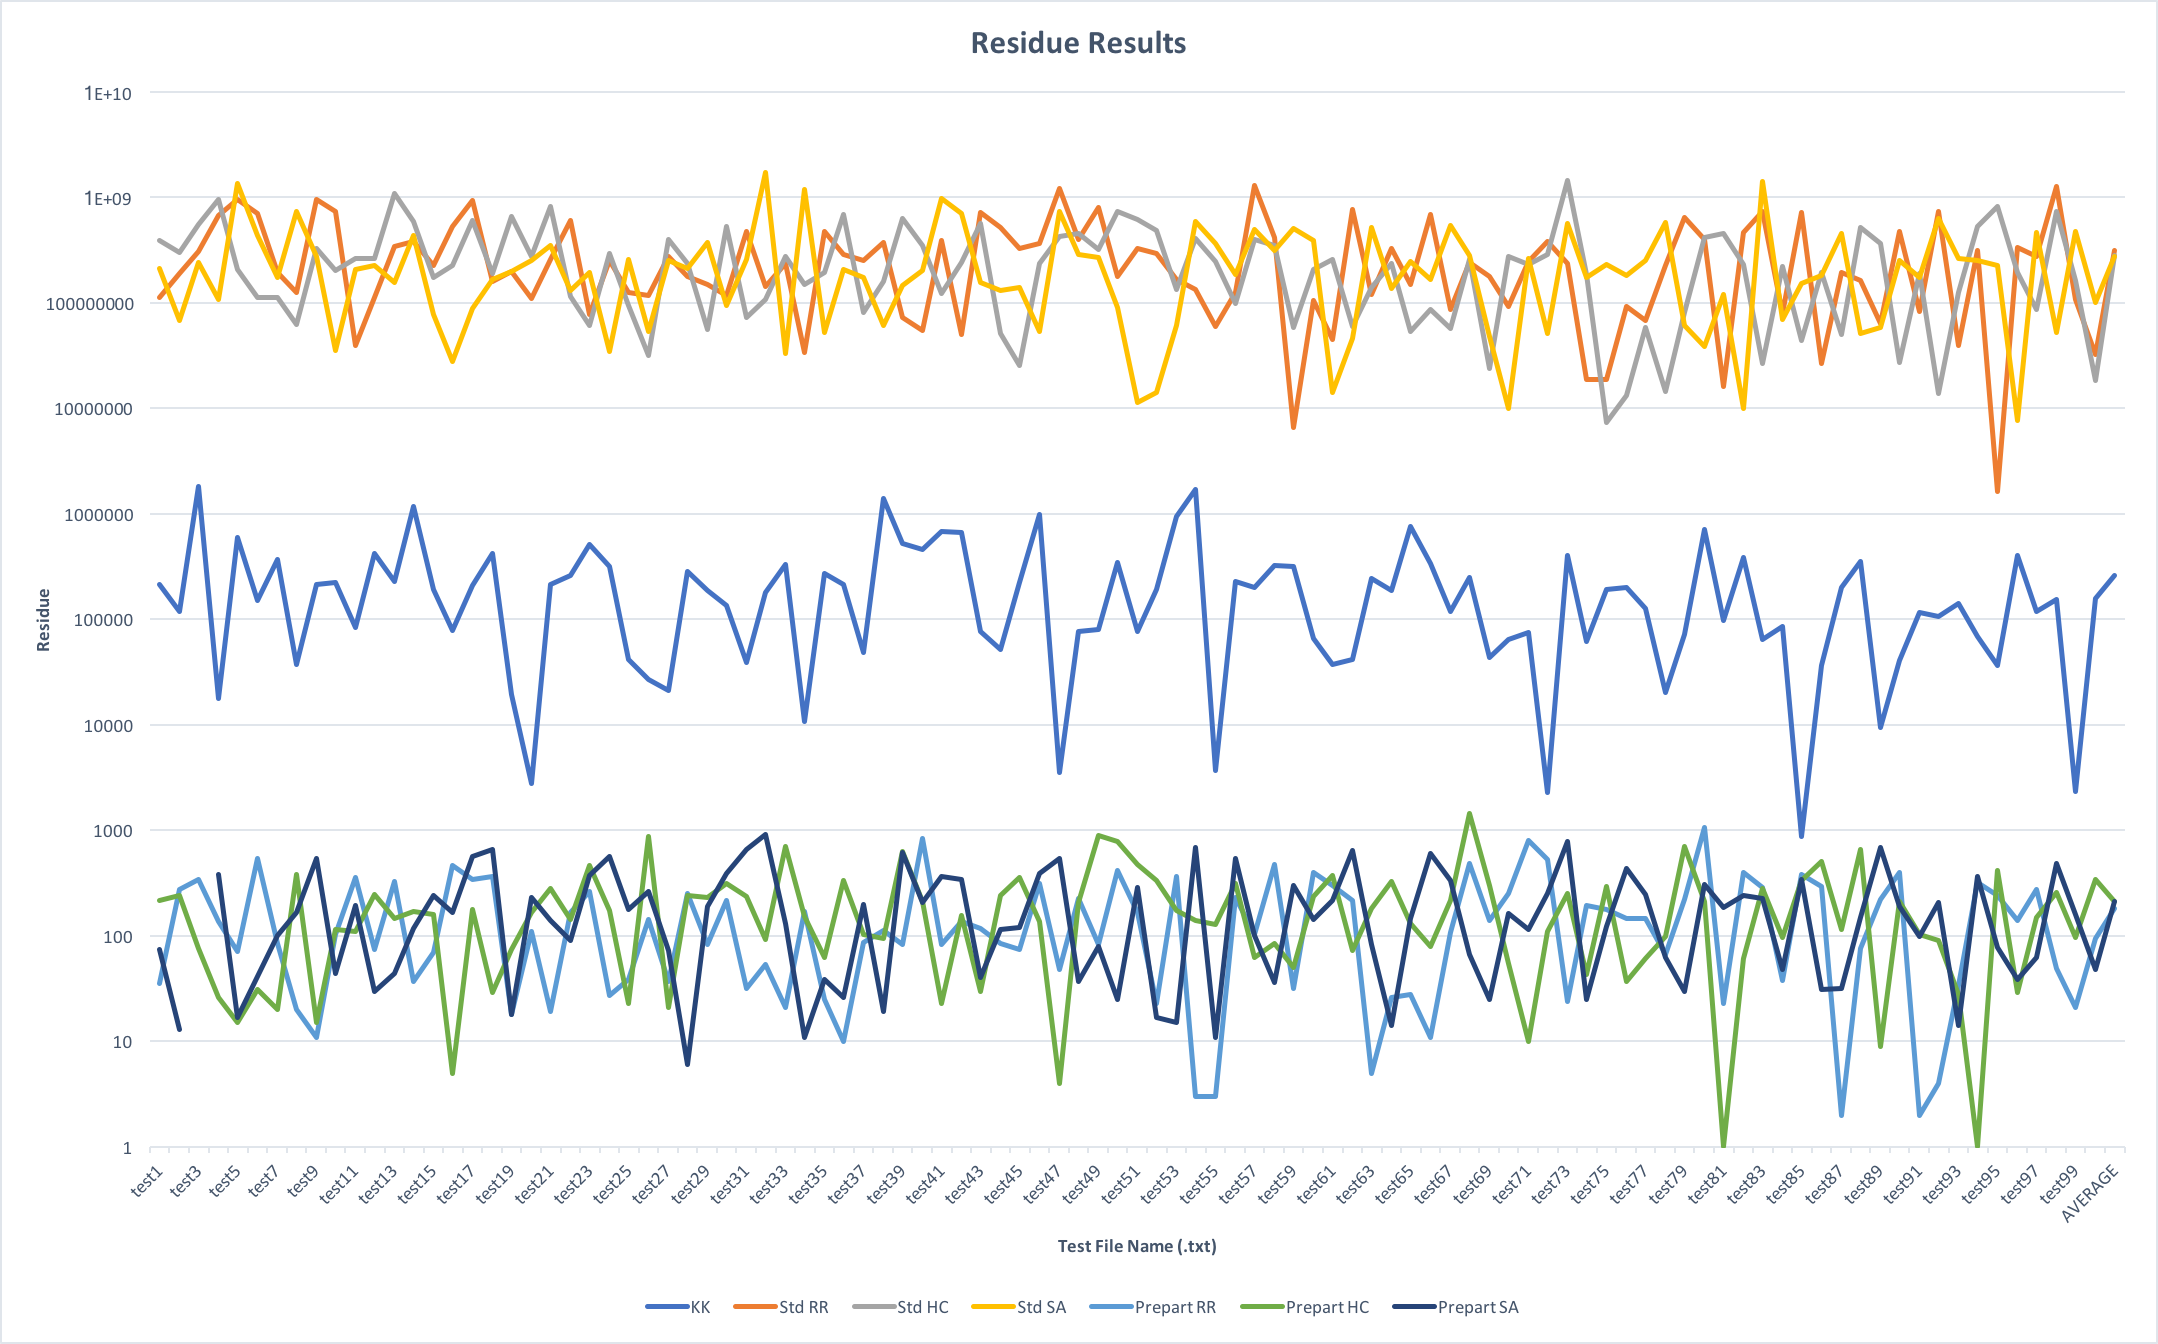
\includegraphics{residueresults} \\
Y-Axis representing residue for 100 trials shows hill climbing (orange line) is overall worse than the other heuristics. Hill climbing has the highest spikes because it gets stuck in local optima.\\

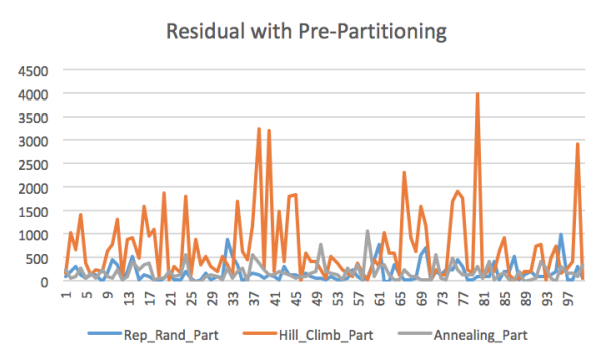
\includegraphics{residualprepart} \\
Y-Axis representing residue for 100 trials are significantly lower for all heuristics. Around the 80th trial, the large spike in hill climbing is due to the solution state getting stuck in a local minima. By and large hill climbing is more likely to perform more poorly than the other methods because it’s performance depends much more on its initial condition and can thus get ’stuck’ in these local optima.\\

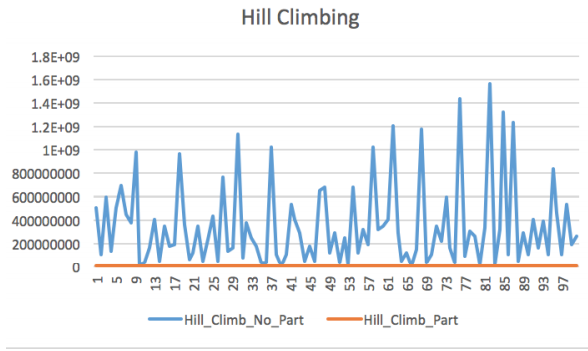
\includegraphics{hillclimbing}\\
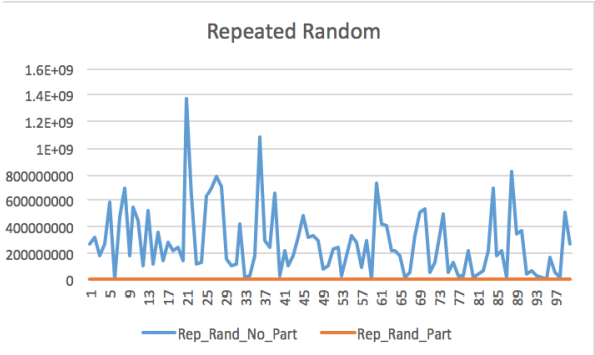
\includegraphics{reprandom}\\
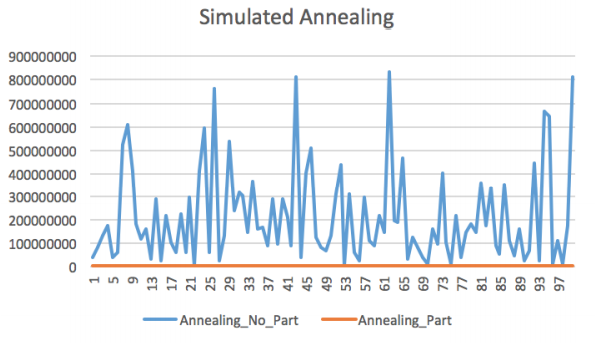
\includegraphics{simann}\\

\section{\textbf{Analysis}}
In a local search algorithm only one state is tracked at a time and each proceeding state it moves to is based on one of many heuristics. While these solutions are not exact, they tend to be close to optimal. \\

The randomized methods (all but KK) had extremely large variation in how well they performed as indicated by the graphs above. The KK algorithm is deterministic in that it always produces the same output (by differencing) regardless of its input type. Of all the methods that I tried, the pre-partitioned random method and the pre-partitioned simulated annealing performed the best by far. The state space for the number partitioning problem is non-convex, meaning the solution is often a local, not global, optima. Therefore, at least for hill climbing methods, there are some initial conditions that will produce a good, but non-optimal solution. Pre-partitioning has a lower residual because it calls KK heuristic on each iteration while the standard algorithm does not. For this reason
the pre-partition heuristics were slower overall but more accurate. Using Karmarkar-Karp is approximately 1000 times better than the non-prepartitioned methods and so because the preparitioned methods rely on it, they are given a huge leg up in terms of finding better parititons. \\

If the solution from the Karmarkar Karp algorithm was used as a starting point rather than a random starting point, there would be significant improvements and much better solutions using the simulated annealing and hill climbing heuristics because using Karmarkar-Karp provides a much better starting place in much less time. In essence, hill climbing or simulated annealing would start much closer to a local maximum than just by guessing one at random. The data showed that that the residual determined by KK is far less than that determined by either hill climbing or simulated annealing with no pre-partitioning. In the repeated random method, random solutions are repeatedly generated to the problem and so any starting point would have no effect on future values unless the KK algorithm returned a residual that was worse than the randomly chosen states, which, as shown by the experiments, almost never happens. Given that low probability, the repeated random method would likely do no better than what KK would start with. \\

Likewise, running KK before the pre-partitioned algorithms would also improve their result,if not with regards to how small a residual they found, then likely in terms of how many iterations it would take to achieve a comparable residual. Instead of beginning with a random prepartition, using the Karmarkar-Karp algorithm would give an assignment of each value. The lower bounds on each solution state are tighter and closer to the optimal because the starting value is more accurate than a randomly generated solution. This would have the largest impact with smaller numbers of trials because there are fewer iterations in which to improve the solution state. \\


\end{document}